\subsection{Deciding at arrival}
\label{sec:arrival}
A policy need not wait for a split: it can rank each block when it is created, against the blocks already
placed. The decision that matters is the same one: where a block with no history ranks against a block
seen once. Every block in a static analysis gets a belief that reads nothing after its own creation;
beliefs are placed in one capacity-constrained assignment. Ranking new blocks among themselves (by
arrival order, by a learned score from session context, or at random) moves the result by at most 5.3
points; moving them ahead of or behind equal-count visible blocks moves it by 14--29 points. An \emph{estimated
prior} replaces that tie rule: at a pseudo-split halfway through the prefix, blocks born after it are
reused before the real split more than blocks already seen once (0.52 against 0.30 on conversation), so
new blocks are placed between count 2 and count 3. It captures 47.0\% and 51.7\% with tier-only actions
(58.2\% and 61.1\% with all actions), and nothing on the synthetic control with tier-only actions. On Alibaba's four Qwen
serving traces~\cite{wang2025kvcachewild} (16-token blocks) it captures 54.3\%, 34.2\% and 45.9\% on three
and 0.0\% on the fourth (thinking), where the prefix rates seen-once blocks above new ones. The direction
the prefix gives is a regularity of these workloads, not a law, and the estimate has to be checked per
workload.

\subsection{Online: recency, and the price of a move}
\label{sec:online}
Static analysis assumes a block, once placed, stays. Replayed online from the heuristic's starting
state with tier-only actions, the same arrival-time arms capture up to 57.3\% when moving a resident is
free. Plain recency does better on the same bill: a multi-tier LRU that moves every accessed block to the
fastest tier captures \textbf{84.5\% and 87.7\%}; caching a block only on its second access captures
$-6.2$\% and $-2.8$\%. Ranking unseen blocks first is a weaker form of recency.

Whether either pays is set by the price of a move. Billed one read plus one write per move, LRU falls to
$-400.5$\% and $-401.4$\%, no replayed arrival arm beats the static heuristic, and the estimated prior
keeps 70\% of its static gain only if a move costs at most 7.3\% and 7.2\% of that price. We timed the
price on one host (an A100 80GB on PCIe Gen4 x16, six runs, a 64\,MiB Mooncake block of an 8B-class
model): a move between GPU and host memory costs 0.75--1.87 times the read-plus-write price, whether it
blocks serving or overlaps it, because the two copy directions did not overlap on this host and a
background move took the link time of a load; a demotion to the host's rotational disk costs 0.90--1.46
times. Every measured price is at least 10 times the estimated prior's break-even.

\begin{figure}[t]
  \centering
  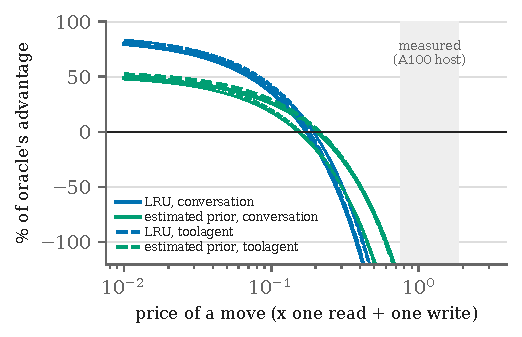
\includegraphics[width=\columnwidth]{fig_price.pdf}
  \caption{Online replay: captured share against the price of a move, as a multiple of one read plus one
  write, for multi-tier LRU and the estimated prior. Thick lines bill every move in full; thin lines write
  every block through to host memory at creation. The shaded band is the range we measured.}
  \label{fig:price}
\end{figure}

The conclusion does not depend on how the hierarchy bills a move. Crediting the serving read to a
promotion, keeping clean lower copies of immutable blocks, or writing every block through to host memory
at creation (the last two without charging the copies' space) leaves LRU at $-401.4$\% to $-353.2$\%,
and no production policy pays once a move costs more than 0.28 of the assumed price; most of LRU's moves
demote blocks just created, which have no copy below. Only on the synthetic control does a moving policy
pay, cache-on-second-hit under the two copy-keeping ledgers (2.6\% and 4.5\%). The remote tier, which
receives most of the arrival arms' online demotions, could not be measured.
